\subsubsection{Gleichgewicht}

Ein Massenpunkt ist im Gleichgewicht wenn die Summe der Kräfte gleich null ist. 

\begin{tabbing}
	\begin{tabu} to \linewidth {l X}
		\toprule
		Kräftegleichgewicht & 
		$\vec{F}_{res} = \vec{F}_1 +\vec{F}_2 + .. + \vec{F}_n \Rightarrow  \sum_{i=1}^{n}\vec{F}_i = \vec{0}
		\Rightarrow  \sum_{i=1}^{n}\vec{M}_i = \vec{0}$ \\
		Massenmittelpunkt & $\sum_{i=1}^{n} \frac{r_i \cdot m_i}{m_ges}$ \\
		\bottomrule
	\end{tabu}
\end{tabbing}

\begin{tabbing}
	\begin{tabu} to \linewidth {l X l}
		Variable & Bedeutung & SI-Einheit \\
		\midrule
		$m_i$ & Massenelemente &  \\ 
		$r_i$ & Ortsvektoren der Massenelemente &  \\ 
		\bottomrule
	\end{tabu}
\end{tabbing}

Die Summe muss mit Vektoraddition ausgerechnet werden. Nach Festlegung eines Koordinatensystems kann mit Komponenten der Vektoren gerechnet werden. In zwei Dimensionen erhalten wir somit zwei Gleichungen und können maximal zwei Unbekannte bestimmen.


\begin{minipage}[h!]{0.5\linewidth}
	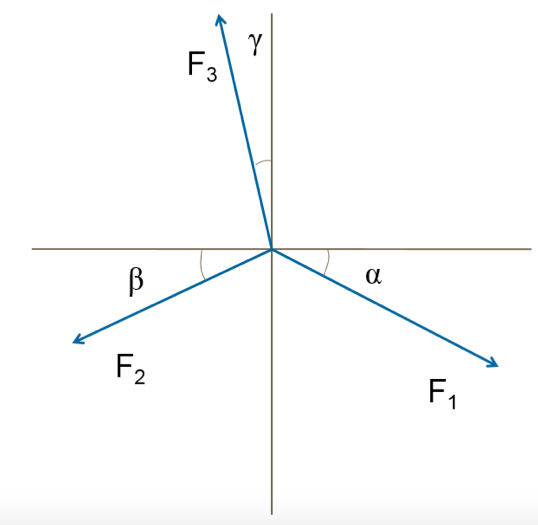
\includegraphics[width=0.7\linewidth]{images/gleichgewicht}
\end{minipage}
\hfill
\begin{minipage}[h!]{0.5\linewidth}
	
	\begin{align*}
	X &: F_1  \cos(\alpha) - F_2  cos(\beta) - F_3 \sin(\gamma) = 0 \\
	Y &: -F_1  \sin(\alpha) - F_2 \sin(\beta) + F_3 \cos(\gamma) = 0
	\end{align*}
	
\end{minipage}

\subsubsection{Schwerpunkt}
Die Gewichtskraft eines Körpers ist gleich der Summe der Gewichtskräfte seiner Teilchen. Die Summe der Gewichtskräfte greift im Schwerpunkt an.

\begin{itemize}
	\item Wenn ein Körper im Schwerpunkt aufgehängt wird, ist er im Gleichgewicht. Somit ist das Drehmoment um den Schwerpunkt = 0
	\item Die Schwerkraft, welche auf einen starren Körper wirkt, kann durch eine Kraft im Schwerpunkt ersetzt werden. $r_p \sum_{i} m_i = \sum_{i} m_i  r_i$
\end{itemize}
